% Header
\renewcommand\evenpagerightmark{{\scshape\small Chapter 6}}
\renewcommand\oddpageleftmark{{\scshape\small Improved RPC investigation and preliminary electronics studies}}

\renewcommand{\bibname}{References}

\hyphenation{}

\chapter[Improved RPC investigation and preliminary electronics studies]%
{Improved RPC investigation and preliminary electronics studies}
\label{chapt6}

	The extension in the endcap of the RPC sub-system towards higher pseudo-rapidity will bring the new detectors to be exposed to much more intense background radiations due to the proximity of the detectors with the beam line. The challenge will be to produce high counting rate detectors with limited ageing rate to ensure a stable operation of the detector over a period longer than 10 years. In Chapter~\ref{chapt4} was discussed the influence of the detector design (number and thickness of gas volumes, OR system, etc...) on the charge deposition and rate capability. Nevertheless, this question can also be adressed from the electronics point of view as a better signal to noise ratio would also mean the possibility to greatly lower the charge threshold on the signals to be detected, allowing to use the detector at lower gain, hence lowering the charge deposition per avalanche in the gas volume. Cardarelli showed that the production of low-noise fast FEE could help decreasing the charge deposition per avalanche at working voltage by an order of magnitude virtually increasing the life expectancy of such a detector in the same way~\cite{CARDARELLI2012}.
	
\section{Extension of the RPC endcap}
\label{chapt6:sec:iRPCs}

\section{FEE candidate for the production of iRPCs}
\label{chapt6:sec:candidates}

	In the context of the CMS Muon Upgrade, two \acf{FEE}s solutions have been considered to equip the new \acf{iRPC}s that are to be added on CMS endcaps. The baseline for the RPC upgrade is based on the PETIROC ASIC, initially for \acf{ToF} applications. A back-up solution is also under study and focusses on a new low-noise preamplifier designed in INFN laboratories in Rome to replace the preamplification stage of the already existing CMS RPC \acf{FEB}.

	The FEEs that are foreseen to equip the new RPCs need to be able to detect charges as small as \SI{10}{fC}. Not only the new electronics need to be fast and reliable, they also should be able to sustain the high radiation the detectors will be subjected to in the region closest to the beam.
	
	\subsection{CMS RPCROC: the RPC upgrade baseline}
	\label{chapt6:ssec:RPCROC}
	
	Designed by Weeroc, a spin-off company from the french OMEGA laboratory, the PETIROC 2A consits in a fast and low jitter 32-channel ASIC originally developed to read-out \acf{SiPM} in ToF applications and that allows for precise time measurements~\cite{PETIROCIEEE,PETIROCTWEPP}. The ASIC uses an AMS \SI{350}{ns} SiGe technology. The block diagram of the ASIC is showed on Figure~\ref{fig:PETIROCASIC}. A 10-bit DAC allows to adjust the trigger level in a dynamical range spanning from 0.5 to a few tens of photoelectrons and a 6-bit DAC to adjust the response of each individual channel to similar a level.
	
	\begin{figure}[H]
		\centering
		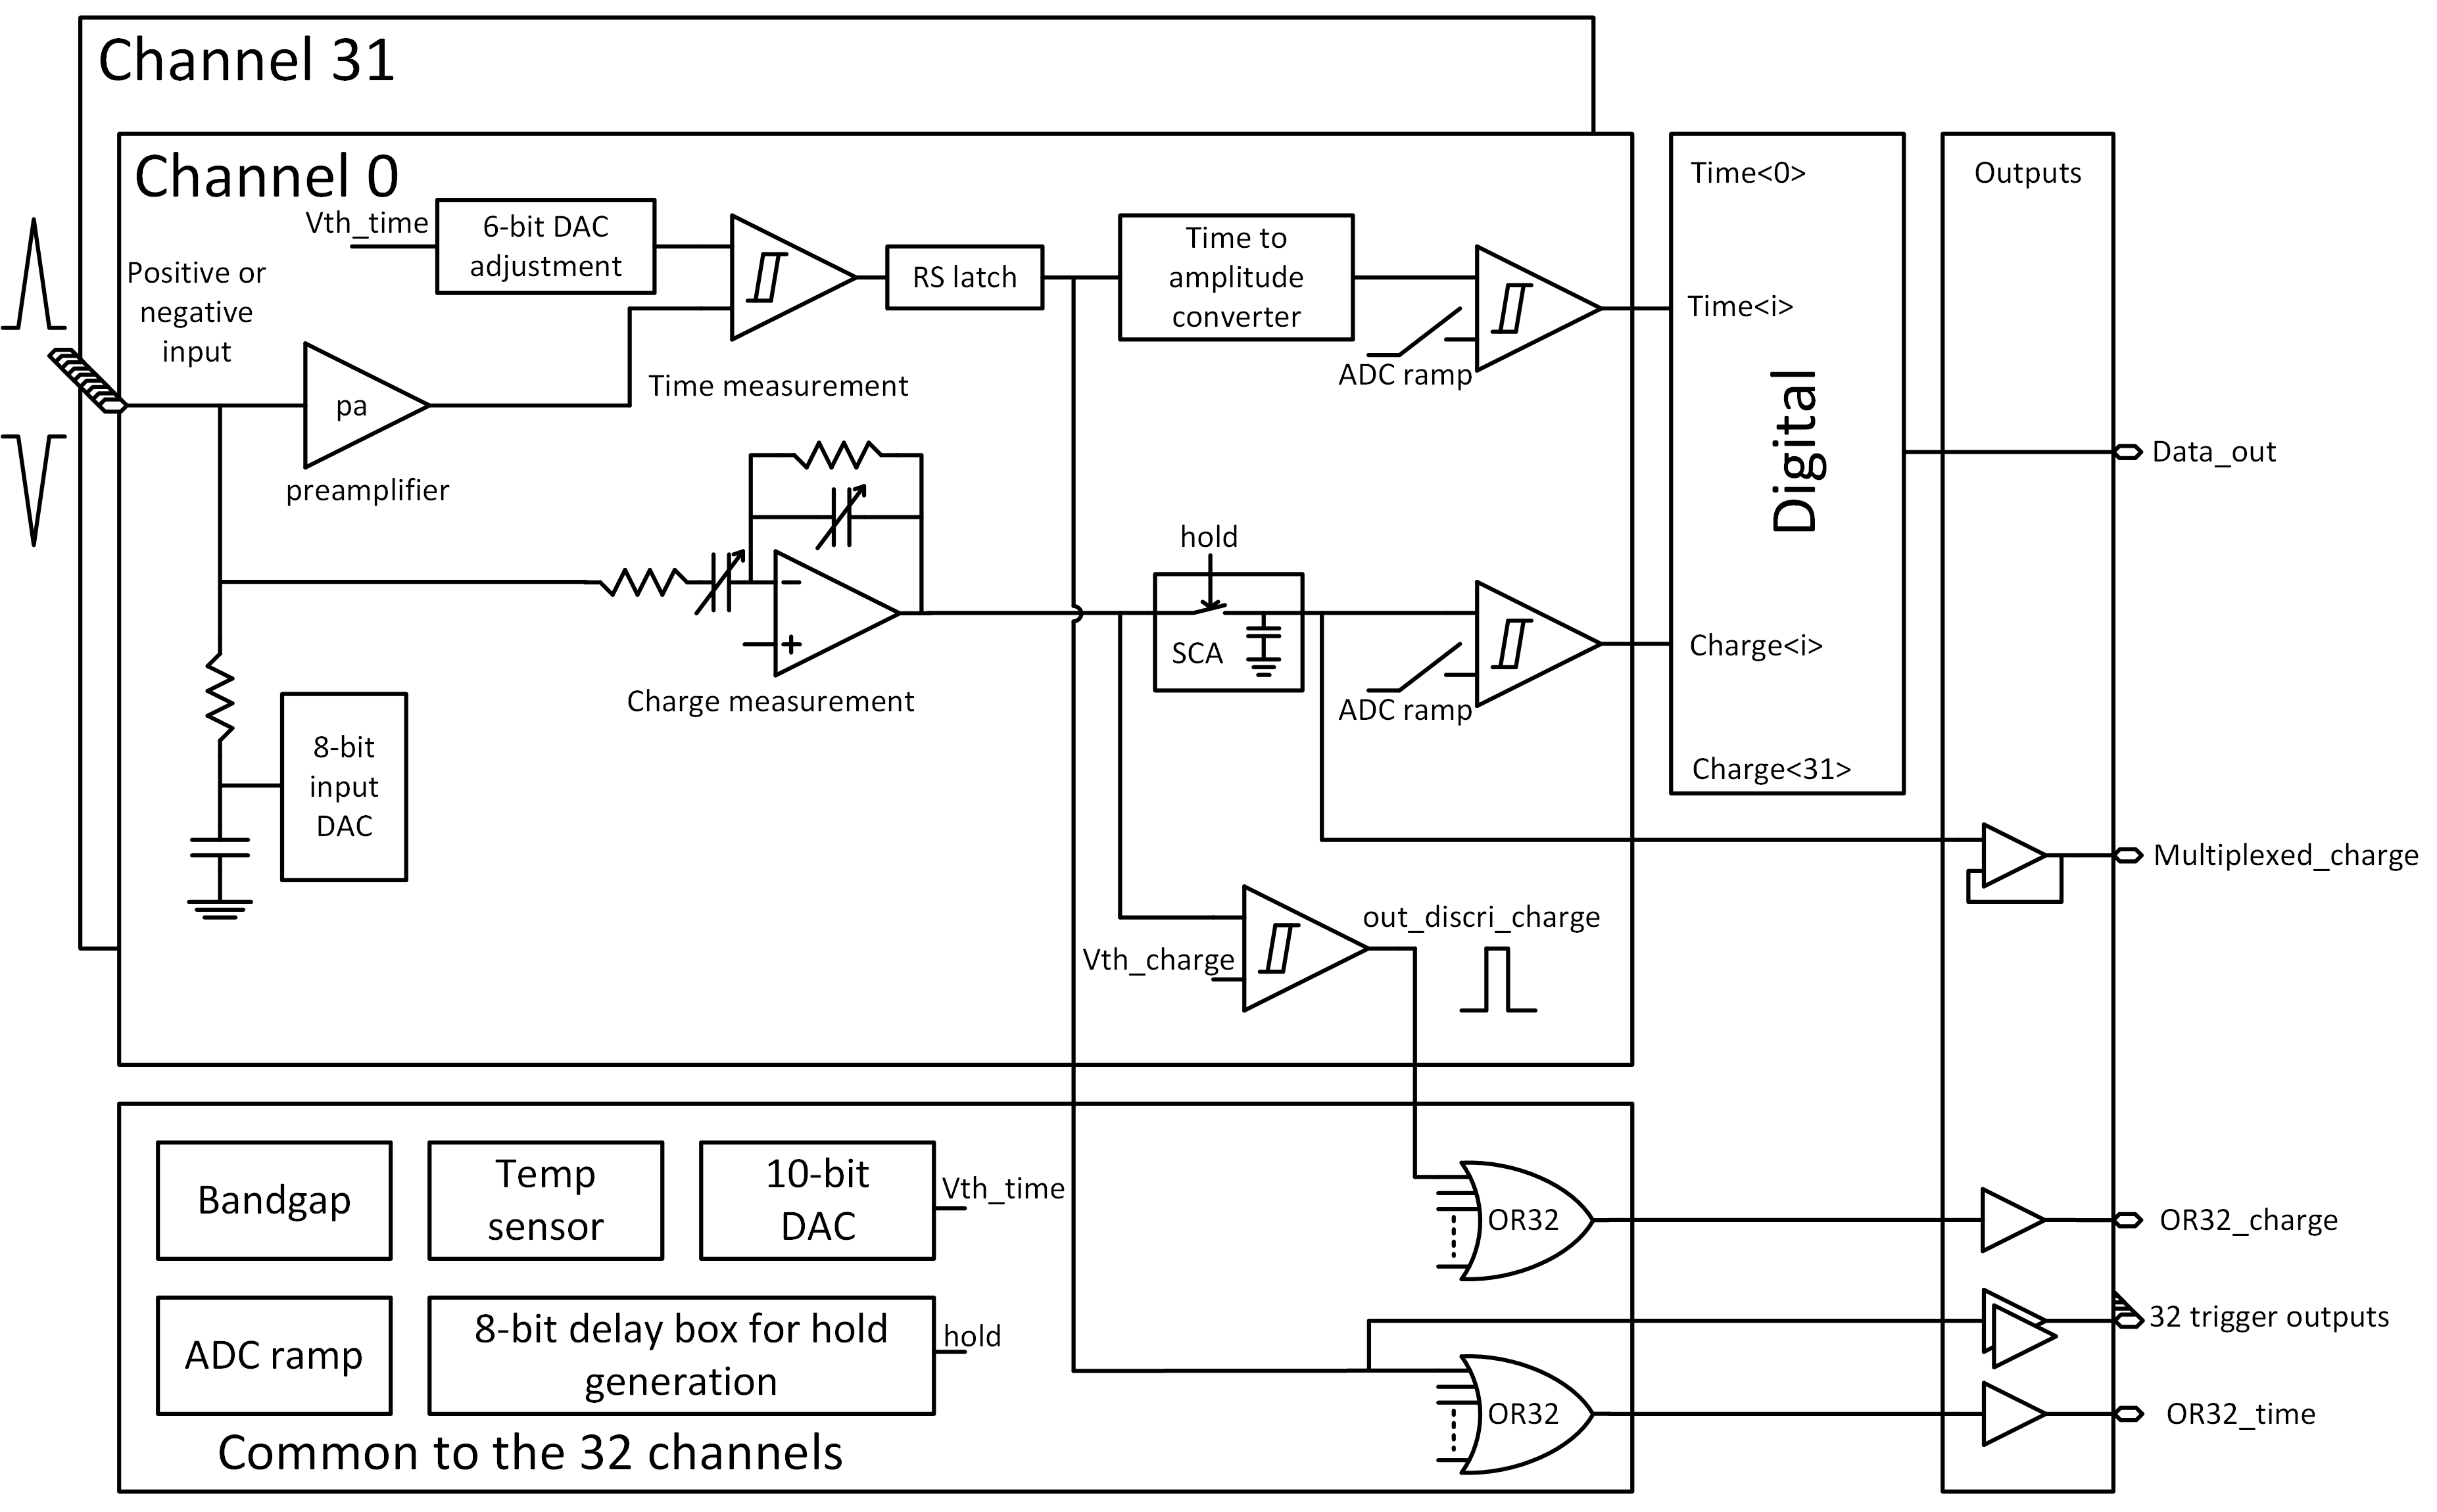
\includegraphics[width = \linewidth]{fig/chapt6/petiroc2.png}\\
		\caption{\label{fig:PETIROCASIC} PETIROC 2A block diagram.}
	\end{figure}
	
	Nevertheless, in order to adapt this ASIC to CMS, modifications were brought to the PETIROC~\cite{PHASEIITP}. In the new CMS RPCROC, the measurement of the charge will be performed by a TimeOverTechnic, taking profit of the capacity the ASIC has in measuring both the leading and trailing edges of the input signals. The dynamic range will be expanded towards lower values to allow for the detection of charges as low as \SI{10}{fC}. Due to the radiation levels that are foreseen at the level of the iRPCs, the SiGe technology will be replaced by the Taiwan Semiconductor Manufacturing Company (TSMC) \SI{130}{nm} CMOS, to increase its radiation hardness. Finally, the number of channels will be increased to 64.
	
	 on which the original SiGe technology will be replaced by CMOS to increase its radiation hardness while keeping fast pre-amplification and discrimination with a very low jitter that can reach less than \SI{20}{ps} if no internal clock is used, as can be seen from Figure~\ref{fig:jitter}. The ASIC is associated with an FPGA which purpose is to measure time thanks to a TDC with a time resolution of 50-100 \si{ps} developed by Tsinghua University and that will provide a measurement of the signal position along the strip with a precision of a few \si{cm} by measuring the signal timing on both ends of the strips. In order to read-out all 96 strips, 3 ASICs and 3 TDCs, each having 64 channels, are hosted on a front-end board attached to the chamber.

	\begin{figure}[H]
		\centering
		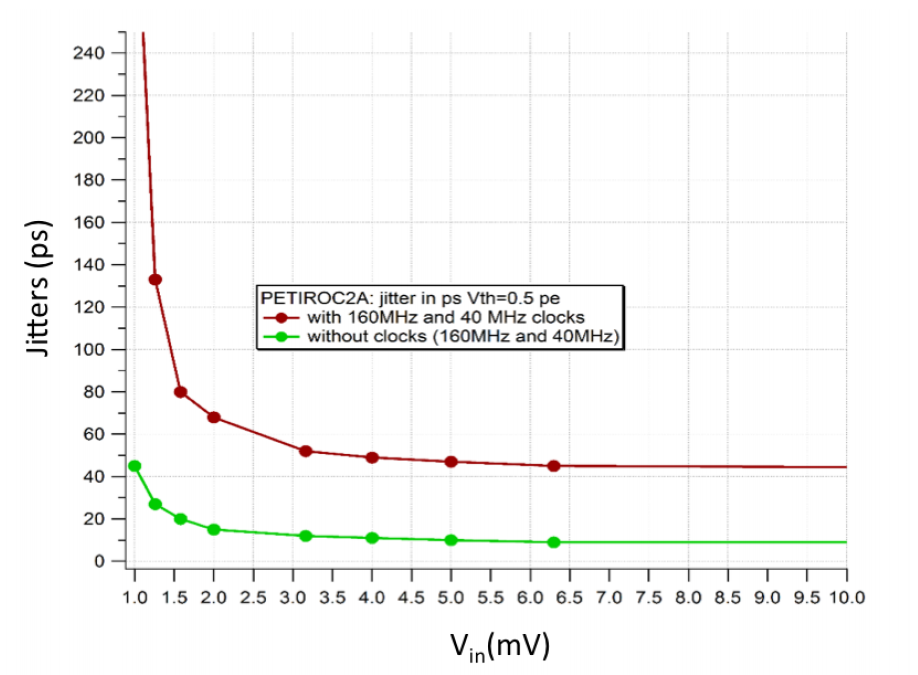
\includegraphics[width=0.8\plotwidth]{fig/chapt6/jitter-PETIROC.png}
		\caption{\label{fig:jitter} The PETIROC time jitter as a function of the input signal amplitude, measured with and without internal clocks.}
	\end{figure}

	\subsection{INFN \acl{FEE}: a robust back-up solution}
	\label{chapt6:ssec:INFN}

\section{Preliminary tests at CERN}

\section{Test }

\clearpage{\pagestyle{empty}\cleardoublepage}